%%%%%%%%%%%%%%%%%%%%%%%%%%%%%%%%%%%%%%%%%
% Short Sectioned Assignment
% LaTeX Template
% Version 1.0 (5/5/12)
%
% This template has been downloaded from:
% http://www.LaTeXTemplates.com
%
% Original author:
% Frits Wenneker (http://www.howtotex.com)
%
% License:
% CC BY-NC-SA 3.0 (http://creativecommons.org/licenses/by-nc-sa/3.0/)
%
%%%%%%%%%%%%%%%%%%%%%%%%%%%%%%%%%%%%%%%%%

%----------------------------------------------------------------------------------------
%	PACKAGES AND OTHER DOCUMENT CONFIGURATIONS
%----------------------------------------------------------------------------------------

\documentclass[paper=a4, fontsize=11pt]{scrartcl} % A4 paper and 11pt font size
\usepackage[top=2.5cm, bottom=2.5cm, left=2.5cm, right=2cm]{geometry}
\usepackage[normalem]{ulem}
\usepackage[T1]{fontenc} % Use 8-bit encoding that has 256 glyphs
\usepackage{fourier} % Use the Adobe Utopia font for the document - comment this line to return to the LaTeX default
\usepackage[english]{babel} % English language/hyphenation
\usepackage{amsmath,amsfonts,amsthm} % Math packages
\usepackage{subfigure}
\usepackage{sidecap}
\usepackage{hyperref}
\hypersetup{colorlinks,urlcolor=blue}

\usepackage{listings}
\lstset{language=BASH}
\usepackage{xcolor}
\usepackage{graphicx}
\graphicspath{ {./images/} }
\usepackage[toc,page]{appendix}

\usepackage{color}

\definecolor{mygreen}{rgb}{0,0.6,0}
\definecolor{mygray}{rgb}{0.5,0.5,0.5}
\definecolor{mymauve}{rgb}{0.58,0,0.82}
\definecolor{light-gray}{gray}{0.95}

\lstset{ %
  backgroundcolor=\color{light-gray},   % choose the background color; you must add \usepackage{color} or \usepackage{xcolor}
  basicstyle=\footnotesize,        % the size of the fonts that are used for the code
  breakatwhitespace=false,         % sets if automatic breaks should only happen at whitespace
  breaklines=true,                 % sets automatic line breaking
  captionpos=b,                    % sets the caption-position to bottom
  commentstyle=\color{mygreen},    % comment style
  deletekeywords={...},            % if you want to delete keywords from the given language
  escapeinside={\%*}{*)},          % if you want to add LaTeX within your code
  extendedchars=true,              % lets you use non-ASCII characters; for 8-bits encodings only, does not work with UTF-8
  frame=single,	                   % adds a frame around the code
  keepspaces=true,                 % keeps spaces in text, useful for keeping indentation of code (possibly needs columns=flexible)
  keywordstyle=\color{purple},       % keyword style
  language=bash,                 % the language of the code
  otherkeywords={*,emacs,sudo, tkmedit, recon-all, freeview, recon-all-go, ship-data, launchfv, ls, FSQC-check, FSQC-summary},           % if you want to add more keywords to the set
  numbers=none,                    % where to put the line-numbers; possible values are (none, left, right)
  numbersep=5pt,                   % how far the line-numbers are from the code
  numberstyle=\tiny\color{mygray}, % the style that is used for the line-numbers
  rulecolor=\color{black},         % if not set, the frame-color may be changed on line-breaks within not-black text (e.g. comments (green here))
  showspaces=false,                % show spaces everywhere adding particular underscores; it overrides 'showstringspaces'
  showstringspaces=false,          % underline spaces within strings only
  showtabs=false,                  % show tabs within strings adding particular underscores
  stepnumber=2,                    % the step between two line-numbers. If it's 1, each line will be numbered
  stringstyle=\color{mymauve},     % string literal style
  tabsize=2,	                   % sets default tabsize to 2 spaces
  title=\lstname                   % show the filename of files included with \lstinputlisting; also try caption instead of title
}

\usepackage{sectsty} % Allows customizing section commands
\allsectionsfont{\centering \normalfont\scshape} % Make all sections centered, the default font and small caps
\makeatletter
\g@addto@macro\@floatboxreset\centering
\makeatother

\usepackage{fancyhdr} % Custom headers and footers
\pagestyle{fancyplain} % Makes all pages in the document conform to the custom headers and footers
\fancyhead{} % No page header - if you want one, create it in the same way as the footers below
\fancyfoot[L]{} % Empty left footer
\fancyfoot[C]{} % Empty center footer
\fancyfoot[R]{\thepage} % Page numbering for right footer
\renewcommand{\headrulewidth}{0pt} % Remove header underlines
\renewcommand{\footrulewidth}{0pt} % Remove footer underlines
\setlength{\headheight}{13.6pt} % Customize the height of the header

\numberwithin{equation}{section} % Number equations within sections (i.e. 1.1, 1.2, 2.1, 2.2 instead of 1, 2, 3, 4)
\numberwithin{figure}{section} % Number figures within sections (i.e. 1.1, 1.2, 2.1, 2.2 instead of 1, 2, 3, 4)
\numberwithin{table}{section} % Number tables within sections (i.e. 1.1, 1.2, 2.1, 2.2 instead of 1, 2, 3, 4)

%----------------------------------------------------------------------------------------
%	TITLE SECTION
%----------------------------------------------------------------------------------------

\newcommand{\horrule}[1]{\rule{\linewidth}{#1}} % Create horizontal rule command with 1 argument of height

\title{	
\normalfont \normalsize 
\textsc{Center for Functional \& Molecular Imaging \\ Georgetown University Medical Center} \\ [25pt] % Your university, school and/or department name(s)
\horrule{0.5pt} \\[0.4cm] % Thin top horizontal rule
\huge Brain Morphometry Analyses in FreeSurfer II:  Troubleshooting \& Manual Editing  \\ % The assignment title
\horrule{2pt} \\[0.5cm] % Thick bottom horizontal rule
}

\author{Made for CFMI training} % Your name

\date{\normalsize 6 November 2015\\ \textit{updated 15 June 2016}} % Today's date or a custom date

\begin{document}

\maketitle % Print the title



%----------------------------------------------------------------------------------------
%	INTRODUCTION 
%----------------------------------------------------------------------------------------

\section{Introduction}  This document is part II of the CFMI guide for brain morphometry analyses in FreeSurfer (FS).  As previously discussed, FS is a remarkable tool for performing automated 3D brain  reconstructions, segmentations and morphometrics (cortical thickness, volume, curvature etc.).  However, sometimes the output of the automated algorithms do not produce quality results and manual user intervention is required.  The purpose of this guide is to establish a standard procedure for manual editing of defects and artifacts that may emerge during the FS processing pipeline.

%----------------------------------------------------------------------------------------
%	OOP
%----------------------------------------------------------------------------------------

\section{Order of Operations} 
\paragraph{Generate QC Summary Profile} FS generates numerous statistics during reconstruction to guide quality correction and assurance. Under \texttt{\$SUBJECTS\_DIR}, there exists for each subject a \texttt{scripts} folder containing the \texttt{recon-all.log} file.  To generate a summary of the QC information from this log, make sure your \texttt{\$SUBJECTS\_DIR} points to the appropriate directory then run the script \texttt{FSQC-summary}:

\begin{lstlisting}
echo $SUBJECTS_DIR 	# confirm subject directory points to right place
outdir=/exports/home/<cfmiuser>/ADS/Projects/data/QC #define directory to store subject QC summary
cd ~/Surfer-gems		# clone this repo using git, see part I of manual
FSQC-summary -sub 149959 -out $outdir
cd $outdir 					# Move to the output directory and view generated files
ls -al
total 48
drwxr-xr-x@  7 shadyeldamaty  staff   238 Jan 13 18:41 .
drwxr-xr-x@ 12 shadyeldamaty  staff   408 Jan 13 18:41 ..
-rw-r--r--@  1 shadyeldamaty  staff   415 Jan 13 18:42 CNR.log
-rw-r--r--@  1 shadyeldamaty  staff  6183 Jan 13 18:42 defects.log
-rw-r--r--@  1 shadyeldamaty  staff   101 Jan 13 18:42 euler-characteristic.log
-rw-r--r--@  1 shadyeldamaty  staff    75 Jan 13 18:42 recon-all-success.log
-rw-r--r--@  1 shadyeldamaty  staff    18 Jan 13 18:42 talairach-spatial-correlation.log
\end{lstlisting}
\lstset{escapechar=\@} % escape lstlisting

After running \texttt{FSQC-summary}, a number of file are generated in the specified output directory:

\begin{description}
\item[recon-all-success.log] This file is written to the QC summary output directory if recon-all was successfully completed for this subject.  The file contains the time and date recon-all was completed for this subject.
\item[recon-all-fail.log] The presence of this file indicates recon-all was not successfully completed.  The file contains the last error message printed to the log before failure.
\item[defects.log] As previously explained in part 1 of this manual, topological defects arise when modeling the cortical surface as a sphere shrunk to the contours of the cortex. Defects in the form of holes and handles are generated by the reconstruction algorithm when a continuous surface cannot be mapped to cortical convolutions. FS contains software to automatically fill in holes and cut handles, however the size and number of defects can seriously impair reconstruction quality.  It is crucially important to review the list of defects for each subject to gauge overall reconstruction quality.  The presence of many defects that contain 1,000 or more vertices indicates the presence of significant artifacts and potential segmentation faults.
\item[euler-characteristic.log]  The euler characteristic is a measure of topological spherical defects and is computed as $2 - 2g$ where $g$ is the number of holes.  This value provides a quantitative measure of image and reconstruction quality.  Less negative numbers (fewer holes) are more desirable.
\item[talairach-spatial-correlation.log]  FS also generates a cross-correlation value between the target talairach atlas and subject image to provide a sense of registration quality.  Values above 0.96 are considered acceptable.
\item[CNR.log]  The contrast to noise ratio (CNR) is the ratio of difference in signal intensities between regions classified as different tissue types vs. the background signal.  FS uses a Gaussian noise model for the estimation of CNR.  Higher values of CNR indicate higher image quality.
\end{description}

These values should be stored and referenced relative to manual QC scoring in order to generate a database of quantitative QC metrics.  We also recommend using the Parallel Connectome Project's Quality Assurance Protocol to further supplement your structural QC metrics.

\paragraph{Batch QC}  The \texttt{Surfer-gems} repository contains a batch program for generating QC files for all subjects listed in a file.  This program will also generate a list of subjects that have failed to complete to allow for easy reprocessing.  You can inspect usage of this script by typing,

\begin{lstlisting}
cd ~/Surfer-gems
FSQC-check -h
\end{lstlisting}

\paragraph{Viewing Subject Data} Once we have a general idea of image quality, we should open and view all relevant images for our subject of interest. Use the \texttt{launchfv} command included in the \texttt{Surfer-gems} repo to make the repetitive task of inspecting a list of subjects much easier:
\newpage
\begin{lstlisting}
export SUBJECTS_DIR="/exports/home/<cfmiuser>/ADS/Projects/data/ads.subjects.tutorial"
launchfv -sub 001
launchfv -h  # see more information on usage using the help flag
\end{lstlisting}

The Freeview command above will allow us to check $A)$ the input anatomical image (T1.mgz), $B)$ the white matter segmentation (wm.mgz), $C)$ the skull-stripped anatomical image (brainmask.mgz) and $D)$ the volume based anatomical segmentation (aseg.mgz).  The pial and white matter surfaces are indicated by the red and blue lines respectively.  

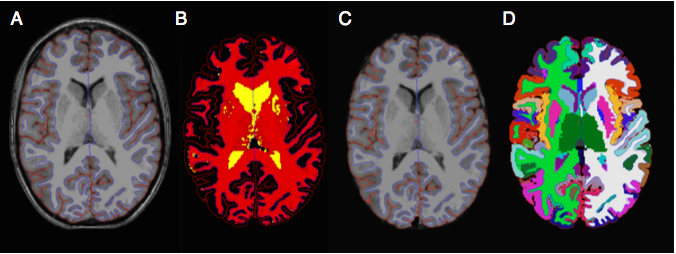
\includegraphics[scale=0.6]{check.png}

We also recommend loading the surface prior to automated topological correction (\texttt{*h.smoothwm.nofix}) and the inflated hemispheres to get a feeling for defects that might have been carried over unto the final surfaces.  These defects will be indicated by the \texttt{defects.log} file generated by \texttt{FSQC-summary}.

\paragraph{important!} \textit{Novice researchers will find great difficulty in finishing checking and editing within the first 30 minutes and it can be quite tempting to over-edit.  However, for an effective editor there are vastly diminishing returns after this time window.  One must build a level of tolerance for some of the errors that are present in automated segmentations.  For instance, a surface defect that appears only in one slice does not require intense user intervention (and is probably not worth the processor time required to reprocess that subject).  The larger errors that persist through many slices are those that will greatly affect our morphometrics.}

\paragraph{Verify Talairach}  The entire processing stream will fail if the subject anatomy is not properly transformed into MNI305 space. This will be indicated by a talairach spatial correlation value < 0.96. See Section \ref{ss:tal} to verify the Talairach transform.  To save time, you may want to also fix any white matter defects before reprocessing the subject with new Talairach transform parameters.

\paragraph{Inspect White Matter} White matter defects provide the biggest source of variance for morphometric analyses.  We must make sure the pial and white matter surfaces follow the anatomy in the structural scan as precisely as possible. To verify the white matter surface, make sure the \texttt{*.white} and \texttt{*.pial} surfaces are selected, deselect \texttt{aseg.mgz} and double-click \texttt{wm.mgz} to bring it to the top with the normalized \texttt{T1.mgz} image as an underlay.  Adjust the opacity of wm.mgz until you can see distinguish between the probability heat map and the structural white matter.  Start from one end of the head and use the \texttt{Page Up/Down} keys down to scroll through the brain paying careful attention to the corona radiata in the coronal and transverse slices.  The white matter segmentation (blue line) should very closely follow the structural scan.  Some deviations from the probability map may be observed.  If the blue line misses a substantial segment of white matter as seen on the structural scan, check the \texttt{wm.mgz} image intensity.  If it is significantly different than 110 then you must use control points to fix it (Section \ref{ss:wser}).  An example in orbitofrontal cortex appears below.  Note the white matter intensity values. \\ 

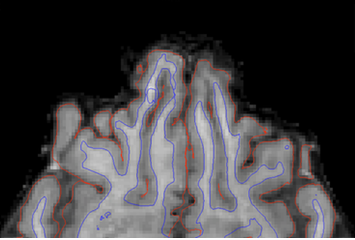
\includegraphics[scale=0.6]{ofc1.png}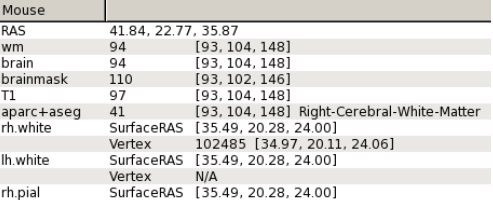
\includegraphics[scale=0.5]{ex1.png}

In the case that gray matter is erroneously segmented as white matter, you must manually delete these voxels from \texttt{wm.mgz} (Section \ref{ss:wse}).  Manual white matter editing is also required in the case that image intensities of excluded white matter segments are not significantly different than 110. \textit{General rule: If a selection of white matter is excluded for 3 or more consecutive slices, edits should be made.  Some WM exclusions are resolved within 2 slices; adding a control point there is not necessary.}

\paragraph{Intensity Normalization Faults}  Low CNR values may indicate low gray-white matter contrast.  Inconsistent and erratic intensity normalization of anatomical T1 scans can lead to faulty tissue-type classifications and substantial inaccuracies in segmentation and anatomical surface generation.  The scan must be thrown out in most cases of low CNR and bad intensity normalization.  An example appears below for A) bad white/gray matter segmentation and B) anomalous white matter segmentation:

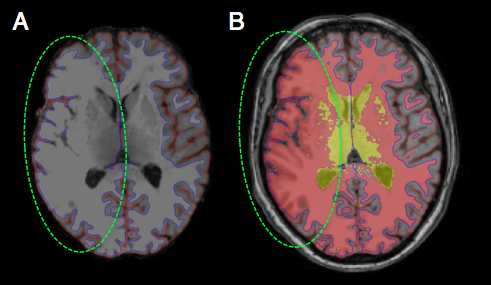
\includegraphics[scale=0.6]{intensity.png}

\paragraph{Perform Gross Inspection} Begin by looking at the 3D pial surface for any obvious topological defects such as skull shards, flattening, exuberant protrusions or general deformations in the surface.  The pial surface should be smooth and follow natural gyral folding patterns.  Make sure that there are no pieces of the brain missing.  If you detect deformities on the pial surface, inspect the brain mask at the location of the troublesome surface by clicking on it and using the \texttt{Page Up/Down} keys to cycle through a transverse, coronal or sagittal view. If large pieces of the skull are retained or pieces of the brain missing, you must fix the skull strip (Section \ref{ss:ss}).  Examples of bad skull strips for A) too aggressive stripping and B) too conservative stripping appear below:

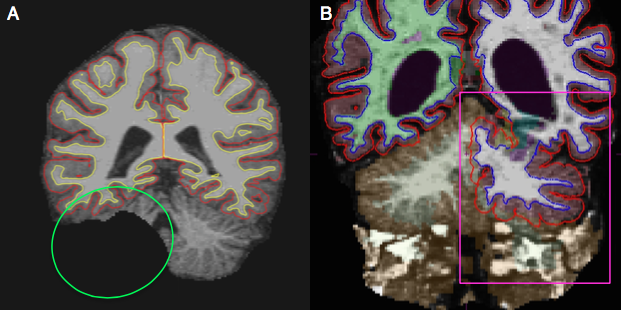
\includegraphics[scale=0.6]{skullstrip.png}

Once the pial surface is verified, you must check the inflated brain for topological defects.  Verify this by looking at \texttt{lh.smoothwm.nofix}.  Turn off the pial and white matter surfaces and look for any holes and bridges in the inflated brain (as in image below).  The curvature should follow natural gyral patterns.  White matter editing is required to perform topological defect correction (Section \ref{ss:wse}). 

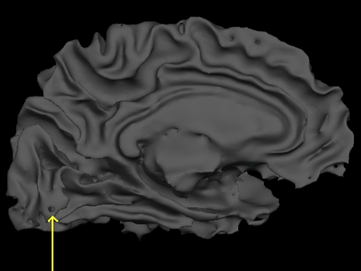
\includegraphics[scale=0.6]{topo.png}

\paragraph{Inspect Pial Surface}  The accuracy of the pial surface depends on the white matter surface reconstruction. If after performing the above edits you still find the pial surface extends into the dura or the skull then you must perform pial surface editing (Section \ref{ss:pse}).  An example of an image requiring pial editing appears below:

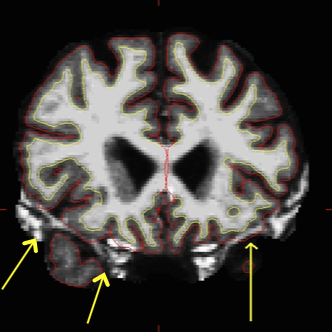
\includegraphics[scale=0.6]{pial.png}

\paragraph{Check Segmentation}  Lastly, we want to check the surface parcellation and volume segmentation.  To verify the segmentation begin by double-clicking the \texttt{aseg.mgz}, lowering the opacity and making sure the macro-structures match up with the structural \texttt{T1.mgz} scan.  If you would like to alter or modify the segmentation follow the instructions in Section \ref{ss:es}.

\paragraph{Summary Table of Edits}  Consult the table below to figure out which edits must be performed.
\paragraph{}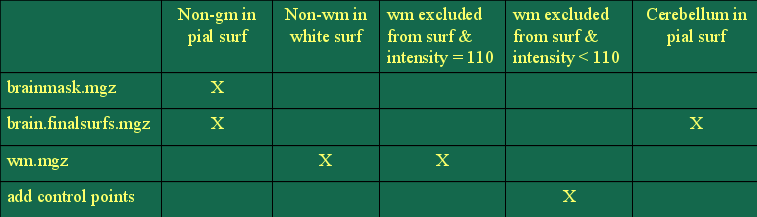
\includegraphics[scale=0.6]{whattoedit}

\paragraph{Additional Notes:}  \paragraph{1.} At no point should the white matter surface intersect with the pial surface. If you have fixed all white matter, pial and topological defects and an intersection is still observed then the subject should not be used for statistical analyses.  There may be a \href{https://www.mail-archive.com/freesurfer%40nmr.mgh.harvard.edu/msg39636.html}{patch} available to address this.
\paragraph{2.} Since the FS processing stages take many hours to complete, it is important to address defects and artifacts early on in the stream.  The various methods for troubleshooting FS output are presented in the order which FS generates the files however sometimes it may make more sense to edit a series of steps before reprocessing the subject.  The user should make the call based on experience.



\section{Defect Correction}
%----------------------------------------------------------------------------------------
% CONTROL POINTS
\subsection{White Matter Segmentation Error}\label{ss:wser} In Part I we discussed that a major challenge of automated brain segmentation is the non-uniformity of white/gray intensity disparity across the brain image due to cytoarchitectural variation, acquisition parameters and artifacts.  Sometimes the intensity normalization step fails to determine the proper intensity for white matter resulting in erroneous white matter segmentation. 

As you scroll through the slices of your subject, you may find incorrect white matter segmentation as indicated by the blue line not properly following the contour of the white matter as shown in Figure 1.1.

\begin{figure}[h]
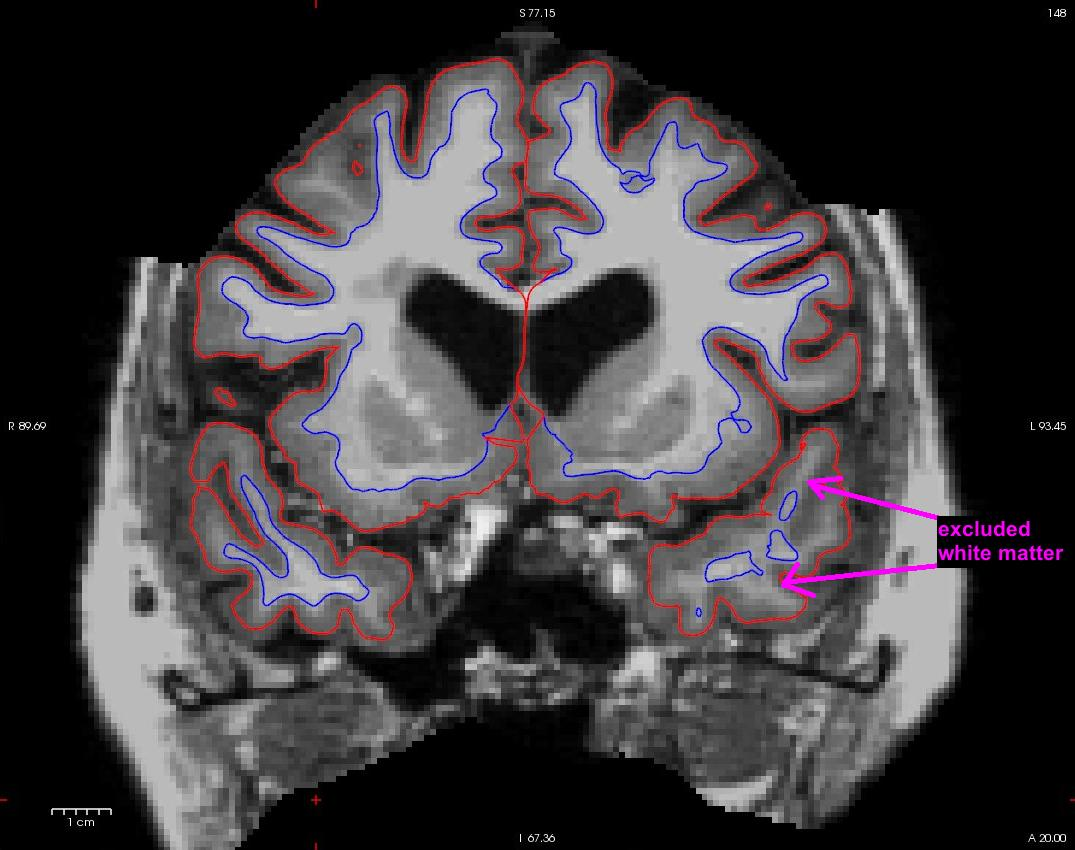
\includegraphics[width=10cm, height=7.5cm]{FS_cp_before}
\caption{\textbf{Incorrect Intensity Normalization Results in White Matter \mbox{Segmentation} Errors.}}
\end{figure}

Mouse over the erroneous area and take note of the intensity value (as shown in the box below the viewing window).  If it is significantly different than 110 then the image was not properly normalized and you can add a \textbf{control point(s)} to renormalize that region. 

\paragraph{Control Points} To add control points you will first need to click on \texttt{File -> New Point Set}, then enter \texttt{control.dat} as the name of the new point set, verify the control points option is selected and the template volume is \texttt{brainmask.mgz}, then click \texttt{OK}. Left-mouse button clicking will create a control point; holding down the \texttt{Shift} button and a Left-mouse button click will delete a control point. 

\paragraph{}Start off with a few control points spread out in your trouble area. You may need to add more. With experience you will be able to determine how many are appropriate, given your specific subject.  As you select control points, they will appear as small green dots. Select a few control points around your trouble areas, space them out throughout the brain and on different slices. You only want to pick points in a region where the white matter intensity is lower than it should be (that is, having a voxel value less than 110).  When you are done, your image should look something like Figure 1.2.
\begin{centering}
\begin{figure}[h]
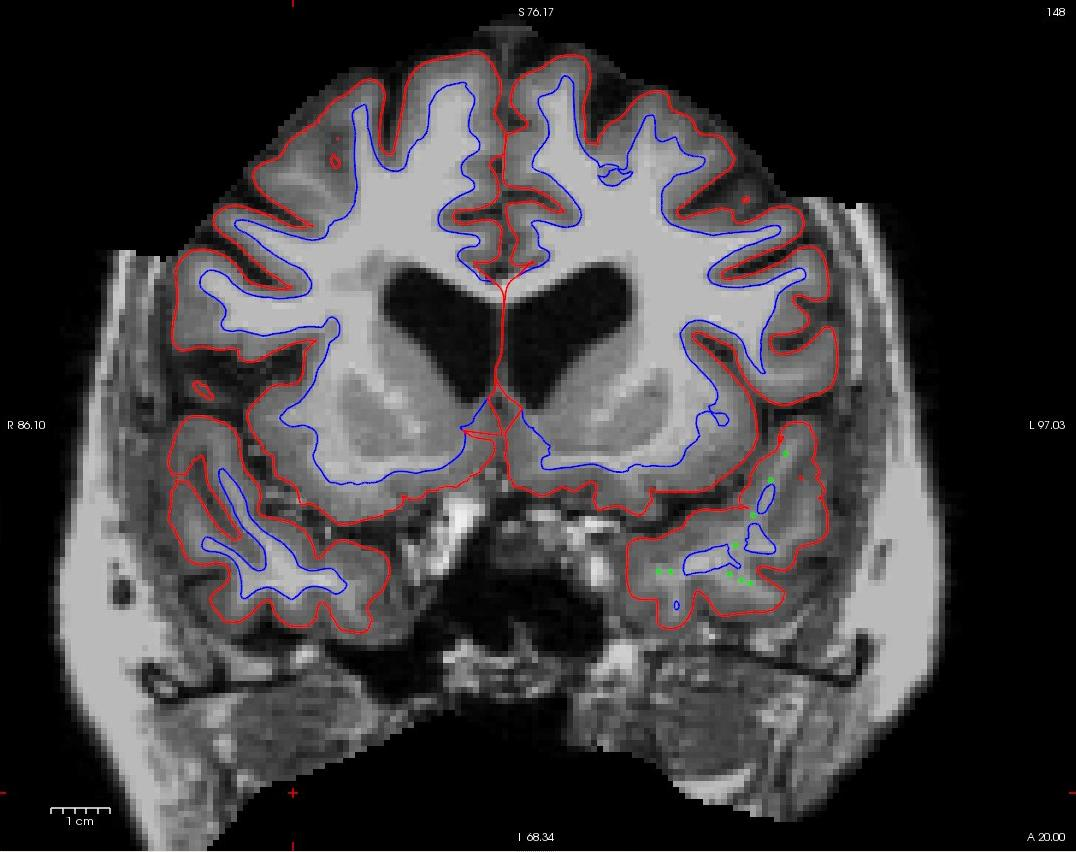
\includegraphics[width=10cm, height=7.5cm]{FS_cp_before_with}
\caption{\textbf{Adding Control Points to Correct Intensity Normalization}}
\end{figure}
\end{centering}
\paragraph{important:} 
\begin{itemize}
\item A control point placed within a region already normalized to 110 will not fix the segmentation error.  If the error is due to a brain lesion, please refer to the procedure for manual white matter edits.

\item Control points should only be added in regions that are definitely white matter (i.e., not in the cortex, cerebellum, brainstem, or outside of the skull).

\item Control points can help recover thin white matter strands that are dark by putting some at the base of the strand.

\item Control points are also useful in areas of very bright intensity (areas significantly greater than 110 in intensity).

\item It is important to be mindful that the control points are three dimensional and extend spherically, meaning they will affect adjacent slices in all directions.  It is best to begin adding control points on the first slice where you observe the issue and add them above every 2-3 slices as you continue navigating through the brain until the local issue is resolved.  \textbf{Do not add control points to every slice}.

\item Sometimes it is necessary to drop control points outside of the pial surface.  Although we typically use control points to extend white matter towards the edge of the pial surface, thus extending both of them, sometimes cortex will be missing in a structure that has higher gray matter thickness and without a direct connection to white matter. This is commonly seen in the frontal and temporal poles and the insula.  In these cases, you should drop control points sparingly, and in a strategic, usually central location that will create the contrast necessary for the pial surface to appropriately capture the structure.

\item Portions of the orbito-frontal cortex are often not captured by the pial surfaced, and will need special attention.  Because of its proximity to the eyes, optic nerves and other bright tissues, voxels in the OFC can sometimes have values well over 120.  Control points brighten voxels to a value of 110, so adding CP's to these voxels will not help in recapturing the surface and may often make the problem worse by brightening other adjacent voxels.
\end{itemize}

After adding the control points, go to \texttt{File -> Save Point Set} or click on the \texttt{Save Point Set} button; enter \texttt{control.dat} as the file name to create a file called \texttt{<subject name>/tmp/control.dat}. Double check that the control points option is selected before saving. Once your control points are saved you can rerun \texttt{recon-all} as follows:
~\\
\begin{lstlisting}[frame=single]
recon-all -autorecon2-cp -autorecon3 -s <subjid>
\end{lstlisting}


~\\ This step can take many hours to run, so submit the job and use the down time to fix up another next subject. Please make sure to have copied the subjects directory to your own user account to prevent over-writing the shared subjects directory and also to speed up processing time.
%----------------------------------------------------------------------------------------
% EDITING WHITE MATTER?
\subsection{Manual White Matter Editing}\label{ss:wse}  Sometimes, the topological fixer fails which leads the white matter surface (colored line in Freeview) to exclude some voxels that are white matter. Simple edits to \texttt{wm.mgz} volume can correct this defect.  After opening your subject in Freeview, you can compare the white matter segmentation with \texttt{wm.mgz} to find places where the white matter was not appropriately filled in.  You can confirm the presence of topological defects by opening \texttt{lh.smoothwm.nofix.surface} and looking for artifact bridges or holes in the 3D surface.  If control points cannot be added then we must use manual editing mode.  Before you begin manual editing, scroll through the volume and note where the artifact begins and ends.
\paragraph{Manual Editing}To begin editing, click on the \texttt{Recon Edit} 
\includegraphics{reconedit.jpg} button on the Freeview tool bar. In the \texttt{Recon Edit} window that pops up, you'll see that the the \texttt{Recon Edit} checkbox is selected, setting the brush value to 255 (yellow) and eraser value to 1. Leave the colormap as heat. Adjust the opacity to make to best accommodate your eyes. Double-check that the \texttt{wm.mgz} volume is on top of and \texttt{brainmask.mgz} is an underlay:  

 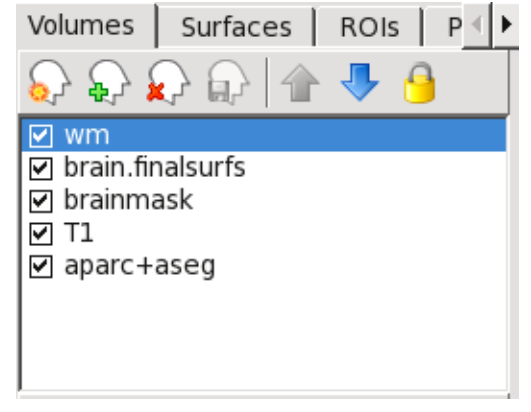
\includegraphics[scale=0.4]{wm-man.png}
 
Use the left mouse button to begin painting in the voxels. Hold down the Shift key while clicking with the left mouse button to delete voxels.  Switch in-between the brain mask and white matter volume to guide your editing.  Only add as many voxels as needed to fix the error. Switch between the coronal, sagittal and horizontal views to check if you need to add more for the white matter to be labelled correctly.
\paragraph{Saving} At any time, you can save the changes you've made to the white matter volume by selecting the \texttt{Save Volume} button or going to\texttt{ File --> Save Volume} while the \texttt{wm.mgz} is highlighted. 
\paragraph{Reprocessing} Once you have made all the edits to the \texttt{wm.mgz} volume, you can run the following command to regenerate the surfaces:
~\\
\begin{lstlisting}[frame=single]
recon-all -autorecon2-wm -autorecon3 -s <subjid>
\end{lstlisting}
%------------------------------------------------
% TAL REGISTRATION
\subsection{Incorrect Talairach Registration}\label{ss:tal} Following intensity normalization FS registers the image to MNI 305 space using the linear Talairach transformation.  The 3x4 affine matrix for the transform is contained in a file called \texttt{talairach.xfm} and can be found under \texttt{<subjid>/mri/transforms directory}.  Although the alignment is automatically checked, it may still fail and it is recommended to check the transform visually.  We use the \texttt{tkregister2} tool to do this:
~\\
\begin{lstlisting}[frame=single]
tkregister2 --mgz --s <subjid> --fstal --surf orig
\end{lstlisting}

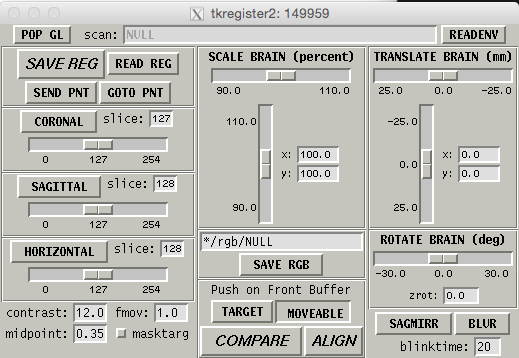
\includegraphics[scale=0.45]{tal1.png}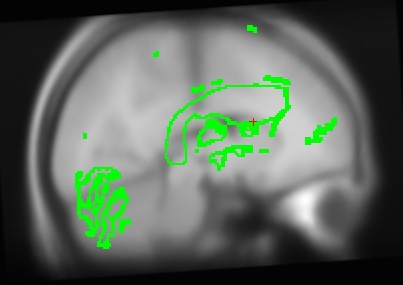
\includegraphics[scale=0.4]{tal2.jpg}

You will see the subject's volume as the \texttt{target} volume and your Talairach volume as a fuzzy \texttt{moveable} volume. The green lines are the \texttt{orig} surface from the subject. This will be the same in both the target and the moveable volumes. It can be turned on and off by clicking in the image window and hitting the \texttt{s} key.

The goal is to stretch, translate, and rotate your \texttt{moveable} volume so that the two brains look as similar as possible, at least along the key anatomical points (anterior/posterior commissures, the temporal lobes in the coronal plane, and the midline cut).  To begin, find the \texttt{fmov:box} in the \texttt{tkregister} toolbar and make sure it is set to \texttt{1.0} and follow the steps below.

\begin{enumerate}
\item Click the \texttt{sagittal} button to switch to a sagittal view, and go to slice 128 by using the slider directly below the sagittal button. In this view you have a good view of the corpus callosum in both the \texttt{moveable} and \texttt{target} volumes use the \texttt{rotate} and \texttt{translate} sliders to align the anterior and posterior commisures.
\item Once you have the corpus callosum aligned as well as possible in the sagittal plane, click the \texttt{horizontal} button to get a horizontal view, and use the slider directly below the horizontal button to go to slice 128. Use \texttt{Ctrl-1} and \texttt{Ctrl-2 }to switch between the two volumes. Use the \texttt{rotate} brain and \texttt{translate} brain buttons to align the midlines of both volumes.
\item Once you are done aligning the brains in the horizontal view, switch back to slice 128 in the sagittal view. Fine tune your rotation and translation again until the corpus callosum is once again aligned in both volumes.
\item Click the \texttt{coronal} button, and go to slice 128. Align the midlines of the brains again in the same way.
\item Continue this way, switching frequently between the \texttt{horizontal}, \texttt{sagittal}, and \texttt{coronal} views, and align the visible brain structures as much as possible in all of the slices. Use the \texttt{scale brain} button as needed to scale the brain in the X and Y direction. Keep in mind that you are working in 3D, not in 2D, so any changes made in one view will affect the other views as well. 
\item Once registration is complete, click the \texttt{save reg} button in the tkregister2 toolbar. You can close \texttt{tkregister2} by closing out the toolbar (but not the viewing window), or by typing \texttt{Ctrl-C} in in the same terminal window.
\end{enumerate}

\paragraph{Reprocessing} Because the Talairach transformation affects everything in the stream it is necessary to rerun the whole process using your new Talairach.  Call \texttt{recon-all} to reprocess the subject.  You \textit{may} want to perform white matter and pial editing before doing this.
~\\
\begin{lstlisting}[frame=single]
recon-all -all -s <subjid>
\end{lstlisting}

\paragraph{Alternative Transforms} If you do not get good results from this method you can use the \texttt{mritotal} utility from the MNI toolset to try an alternative algorithm for the Talairach transform.  This does not work in all cases.
~\\
\begin{lstlisting}[frame= single]
recon-all -s <subjid> -talairach -use-mritotal -tal-check \
						-clean-tal
\end{lstlisting}
%----------------------------------------------------------------------------------------
% SKULL STRIPPING

\subsection{Bad Skull Stripping}\label{ss:ss} Occasionally, the skull stripping step either removes more than just the skull, causing part of the brain to be removed or leaving behind portions of the skull. These problems heavily influence deformities in later processing stages.  We can fix a bad skull strip by either  manually editing the volumes or by adjusting input parameters to the skull stripping step, and running again until a good result is obtained. Often the sagittal view reveals skull strip failures. Note that the inflated 3D surface is a less reliable gauge of skull strip failure unless large portions of the brain are missing, or lots of skull is retained. We will use Freeview to inspect the subject for skull stripping errors:
~\\
\begin{lstlisting}[frame=single]
subjid=<subjid>
launchfv 
\end{lstlisting}
Look for parts of the brain or cerebellum that might have been omitted in \texttt{brainmask.mgz} compared to \texttt{T1.mgz}.  In general there are two ways to fix a volume when there is something missing from the cortex or cerebellum, you can clone the missing pieces in manually or you can adjust the parameters of \texttt{mri\_watershed} to do it automatically.  When large pieces of the brain/skull are missing/included it is best to adjust the parameters of \texttt{mri\_watershed}.

\paragraph{Adjusting Watershed Parameters} The watershed algorithm is used during the skull stripping step to find a boundary between the brain and skull. The \texttt{mri\_watershed} program uses a default preflooding height of 25 percent. If we want the algorithm to be more conservative (i.e. if part of the brain has been removed), you will want to make that number larger than 25. If you want the algorithm to be more aggressive (i.e. part of the skull has been left behind), you will want to make the height less than 25. There aren't any hard and fast rules about how to select your height value. You can adjust the preflooding height by passing the following flag to recon-all:
~\\
\begin{lstlisting}[frame=single]
recon-all -skul@ls@trip -wsthresh <h> -clean-bm -s <subjid>
\end{lstlisting}
~\\
where <h> is replaced with the preflooding height you'd like to use and <subjid> is replaced with your subject. The clean-bm flag is used to instruct recon-all to write over the old \texttt{brainmask.mgz} volume with your new edits. If you do not use this flag your changes will not take effect.  After this process is completed open your output volume along with the original T1 volume to verify the new skull stripping is correct.
~\\
\begin{lstlisting}[frame=single]
subjid=<subjid>
launchfv 
\end{lstlisting}
\paragraph{dura cutting like a g} The fastest way to remove extra pieces of dura left in the brain mask is to use the -gcut flag followed by manual editing.  This flag removes any extra dura that could influence the surfaces.
~\\
\begin{lstlisting}[frame=single]
recon-all -skul@ls@trip -clean-bm -gcut -s <subjid>
\end{lstlisting}
Be sure to carefully inspect your data when using \texttt{-gcut.}  In particular check the edges of the gray matter and cerebellum for liberal cutting. You can open the \texttt{brainmask.gcuts.mgz} volume in Freeview to see which voxels were removed with \texttt{gcut}. After the bad skull strip has been improved, you can run the following command to regenerate Freesurfer output based on the new \texttt{brainmask.mgz}.
~\\
\begin{lstlisting}[frame=single]
recon-all -autorecon-pial -s <subjid>
\end{lstlisting}
%----------------------------------------------------------------------------------------
% PIAL SURFACES
\subsection{Correcting Pial Surfaces}\label{ss:pse}
As previously explained in Part I, the pial surface is created by expanding the white matter surface so that it closely follows the gray-CSF intensity gradient as found in the \texttt{brainmask.mgz} volume. Once an accurate white surface is created then you can work on correcting the pial surface, if needed. \textbf{The pial surface boundary and white matter surface boundary should not cross.} After the pial surface has been generated, it's a good idea to visually check it for defects that may have been created during automatic topology fixing. To check the pial surface, it may be loaded into Freeview and viewed along with the \texttt{brainmask.mgz} volume. If the surface appears not to follow the gray-CSF boundary in the volume, edits may be required. To inspect and edit a subject's pial surface, begin with launching Freeview (as done previously) and use the \texttt{PageUp} and \texttt{PageDown} keys to go through the volume slice by slice.  Look for any pieces of dura that might have been included in the pial surface.  Double-click on \texttt{brainmask.mgz} on the list of volumes in the top left panel to make sure it is selected.  ~\\ Next click on the \texttt{recon Edit} button 

\includegraphics{reconedit.jpg}
to bring up the following window: ~\\~\\
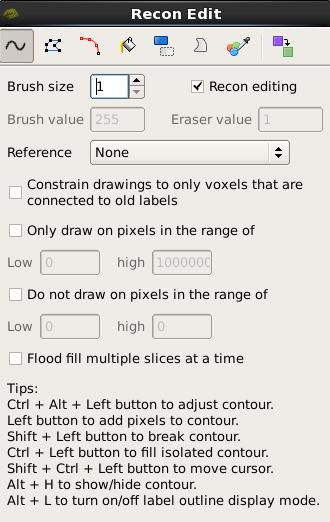
\includegraphics[scale=0.6]{reconeditingwindow.jpg} 
\paragraph{} Make sure that the \texttt{recon editing} box is checked and set the brush size to an appropriate value for the scale of your edits.  In Recon editing mode the \texttt{brush} value and \texttt{eraser} value are set to \texttt{255} and \texttt{1}, respectively. Make sure the first option, \texttt{Freehand}, a squiggly panel at the top-left, is selected and you're ready to make your edits. Find a place in the image where the dura is causing errors in the segmentation. 
\paragraph{}Double check that the \texttt{brainmask.mgz} (not the \texttt{T1.mgz}) is selected and highlighted in the side panel listing all the volumes. You only want to make edits to the brain mask. Hold down the Shift key and use the left mouse button to delete the voxels. It is not necessary to completely remove the dura to get an adequate pial surface, but it is good to do so until you are more familiar with manual editing. Continue on the other slices until the dura is removed. \texttt{Ctrl-Z} and the \texttt{Undo} button at the top in Freeview allows you to go back and undo as many edits as you like.  
\paragraph{}At any time, you can save the changes you've made to \texttt{brainmask.mgz}  by selecting \texttt{Save Volume} in the Freeview \texttt{File menu} or by clicking the \texttt{Save Volume  -> save.jpeg} button. Make sure the \texttt{brainmask.mgz} is the one highlighted while saving if you have the \texttt{T1.mgz} open at the same time. You can check your result by viewing the \texttt{brainmask.mgz} volume in the subject directory directory.
\paragraph{Regenerating the Surface} When you are finished editing the voxels, you will need to regenerate the surfaces. Since the white matter hasn't been changed, you don't need to resegment the volume. You can regenerate the pial surface with:
~\\
\begin{lstlisting}[frame=single]
recon-all -autorecon-pial -s <subjid>
\end{lstlisting}
%----------------------------------------------------------------------------------------
% FIXING TOPOLOGY
% same as white matter editing??
%----------------------------------------------------------------------------------------
% EDITING SEGMENTATIONS
\subsection{Editing Segmentations}\label{ss:es} A segmentation is a volume whose values represent an index of an anatomical structure or label to which the corresponding voxel in the main anatomical volume belongs. The structures are listed in a lookup table. This table also specifies the colors the structures should appear in, and is more commonly called a color table.  
\paragraph{Loading}Once you have loaded a brain mask or T1 volume, you can load a segmentation volume by clicking the \texttt{Load Volume} button, clicking on the yellow folder and then scrolling in the \texttt{mri} folder until you find the segmentation file you want. Click on it and then \texttt{Open}, then click \texttt{OK}. At first the segmentation will obscure the brain volume, but if you change the \texttt{Color map} field to \texttt{Lookup Table} and move the \texttt{Opacity} slider to around .25, you will be able to see both the brain and segmentation.
\paragraph{Display Options} Segmentations are drawn as a colored overlay in the \texttt{Display Window}. The colors are defined in the color lookup table file specified at load time. The opacity of the overlay can be configured by moving the \texttt{Opacity} slider while the aseg is on top and highlighted. You may also enter the desired number and hit enter. The overlay can be hidden by unchecking the check box next to aseg in the volumes tab. You can use that or \texttt{Alt-C} to toggle back and forth between the brain and aseg to check its accuracy. Hovering you cursor over a certain label or clicking will display the segmentation label value and name next to aseg in the \texttt{Cursor} and \texttt{Mouse} windows below the main viewing window.
\paragraph{Editing} A segmentation can be edited by clicking on the \texttt{Voxel Edit} button above the volumes tab. In the \texttt{Voxel Edit} window that pops up, you can change your brush size, then verify that the freehand tool is selected and that \texttt{Recon Editing} is \textbf{not} selected, then you can begin editing. When the segmentation volume is highlighted and the \texttt{Lookup Table} selected for the color table, you can scroll through all the different label values in the list to the left of the viewing window. You can click on one to use that color. If, for example, the Left-Pallidum is overlabeled into the white matter, you can select 2 Left-Cerebral-White-Matter, then using your left mouse button, click on the voxels in the segmentation volume you wish to change to the white matter label. If you change too many or make a mistake, you can press \texttt{Ctrl-Z} as many times as you like to undo your last edits. You can also hold down the Shift key while clicking with your left mouse button to delete voxels, but you would likely have to replace them with another label. Erasing voxels in a segmentation volume changes them to a value of \texttt{O}, or Unknown.

\paragraph{} If you're creating a new segmentation, you can outline the structure you wish to label, making sure there are no gaps in the outline, then hold down the \texttt{Crtl} key and click the left mouse button. This will fill the outline with the new label value. If it fills the whole slice, you have not completely closed the outline. These two functions are essentially a paint brush and paint fill. You will have to do this in each slice you wish to label a structure.  At any time you can change to "outline mode" for the segmentation by pressing \texttt{Alt-L}. This also helps for viewing the brain and segmentation at the same time. In the popup \texttt{Voxel Edit} window, there is also a \texttt{Color Picker} button you can select and then click on a label on your segmentation to speed up changing from one label to another. You will have to again click on the freehand button to continue and use that color to draw.

\paragraph{saving and reprocessing} To save changes to a segmentation, make sure the segmentation is highlighted then go to \texttt{File->Save Volume} to overwrite the original segmentation volume or \texttt{File->Save Volume As}... to specify a new volume, such as an .mgh or .mgz volume, or an empty directory in which to save a volume. After you have saved all of your edits, you can create the final surfaces with the command:
~\\
\begin{lstlisting}[frame=single]
recon-all -autorecon2-noaseg -s <subjid>
\end{lstlisting}
%----------------------------------------------------------------------------------------
% Appendix?
%----------------------------------------------------------------------------------------

\end{document}